\documentclass[../index.tex]{subfiles}

\begin{document}
    % 4.1
    \section{Thiết kế kiến trúc}
    Như đã phân tích ở mục 1, chúng ta sẽ sử dụng kiến trúc Microservices cho hệ
    thống diễn đàn trực tuyến.

    \begin{figure}[H]
        \centering
        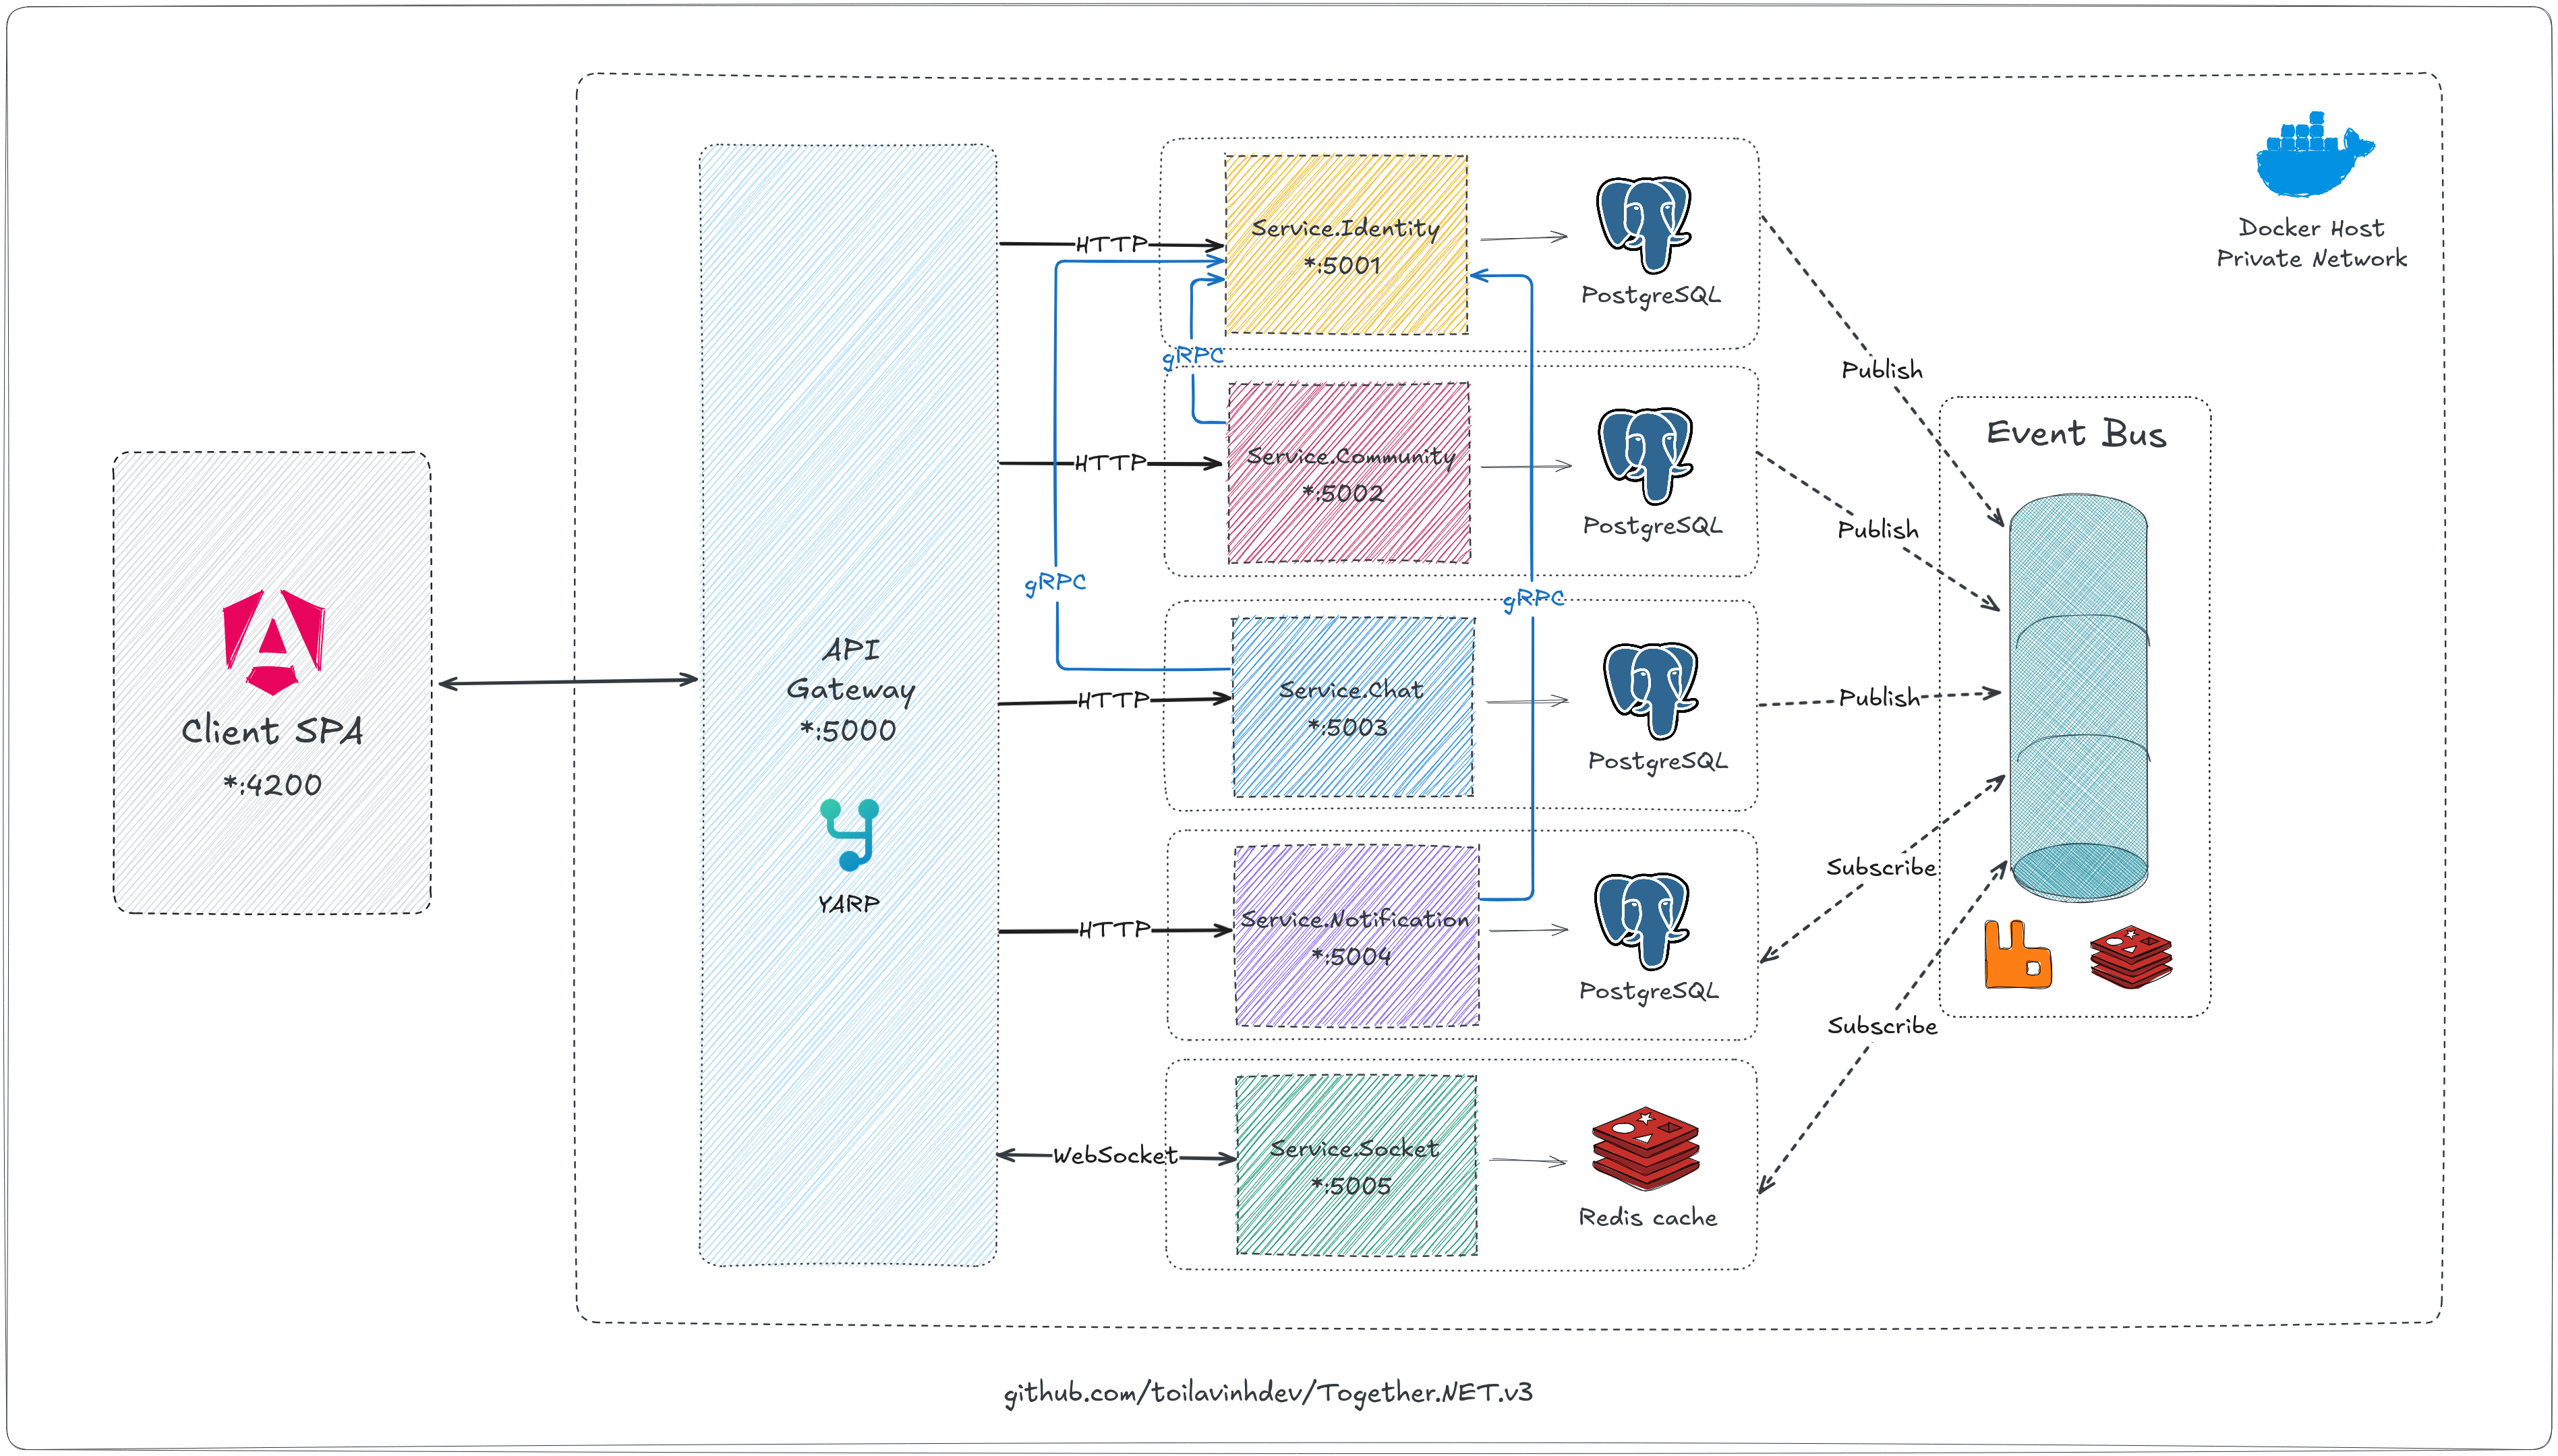
\includegraphics[width=0.95\linewidth,angle=270,scale=1.4]{../figures/architecture.png}
        \caption{Thiết kế kiến trúc hệ thống dự án diễn đàn trực tuyến}
        \label{fig:architecture}
    \end{figure}

    \textbf{Sơ đồ tương tác}:
    \begin{enumerate}
        \item Client gửi yêu cầu đến API Gateway.

        \item API Gateway định tuyến yêu cầu đến microservice phù hợp.

        \item Microservice xử lý yêu cầu, giao tiếp với nhau bằng gRPC và có thể
            phát sinh các sự kiện.

        \item Các sự kiện được gửi đến Event Bus.

        \item Các microservice khác đăng ký sự kiện sẽ nhận và xử lý.

        \item Kết quả được trả về cho client qua API Gateway.
    \end{enumerate}

    Hệ thống có sử dụng YARP làm API Gateway. API Gateway là một công cụ trung gian,
    đóng vai trò như một "cổng vào" duy nhất cho các ứng dụng khách truy cập vào
    nhiều dịch vụ backend khác nhau trong một hệ thống, đặc biệt là trong kiến trúc
    microservices của dự án. Nó hoạt động như một máy chủ reverse proxy, nhận tất
    cả các yêu cầu API bao gồm HTTP/HTTP2 và WebSocket, sau đó phân phối và xử
    lý các yêu cầu đó đến các microservice phù hợp.

    Angular có vai trò như là máy khách của ứng dụng sẽ giao tiếp trực tiếp với
    API Gateway thông qua giao thức HTTP/HTTP2 hoặc WebSocket

    Các microservice trong hệ thống được triển khai trong các container Docker,
    giúp cách ly các dịch vụ, đảm bảo tính nhất quán và dễ dàng quản lý. Mỗi
    microservice có một cơ sở dữ liệu riêng (PostgreSQL hoặc Redis) để quản lý
    dữ liệu của mình, tạo điều kiện cho việc phát triển độc lập và mở rộng.

    Từ các khảo sát và phân tích nghiệp vụ ở chương 2, ta chia hệ thống thành 5
    microservice:
    \begin{enumerate}
        \item \textbf{Service.Identity}: Một máy chủ ủy quyền, quản lý người
            dùng và vai trò.

        \item \textbf{Service.Community}: Quản lý toàn bộ nội dung của diễn đàn.

        \item \textbf{Service.Chat}: Quản lý chức năng chat giữa các thành viên

        \item \textbf{Service.Notification}: Quản lý chức năng thông báo

        \item \textbf{Service.Socket}: Quản lý các kết nối WebSocket, hỗ trợ
            realtime cho ứng dụng.
    \end{enumerate}

    Dự án có sử dụng gRPC làm cơ chế giao tiếp đồng bộ chính giữa các
    microservices. Mỗi microservice sẽ định nghĩa một giao diện gRPC, mô tả các
    phương thức mà các dịch vụ khác có thể gọi đến.

    Cuối cùng là Event Bus đóng vai trò quan trọng trong việc truyền tải các sự
    kiện giữa các microservices. Khi một sự kiện xảy ra ở một microservice, nó
    sẽ được phát trên Event Bus và các microservice khác đăng ký sự kiện đó sẽ
    nhận được và xử lý, tạo nên một cơ chế thông báo và cập nhật dữ liệu hiệu quả.

    % 4.2
    \section{Thiết kế cơ sở dữ liệu}
    % 4.2.1
    \subsection{Service Identity}
    \begin{figure}[H]
        \centering
        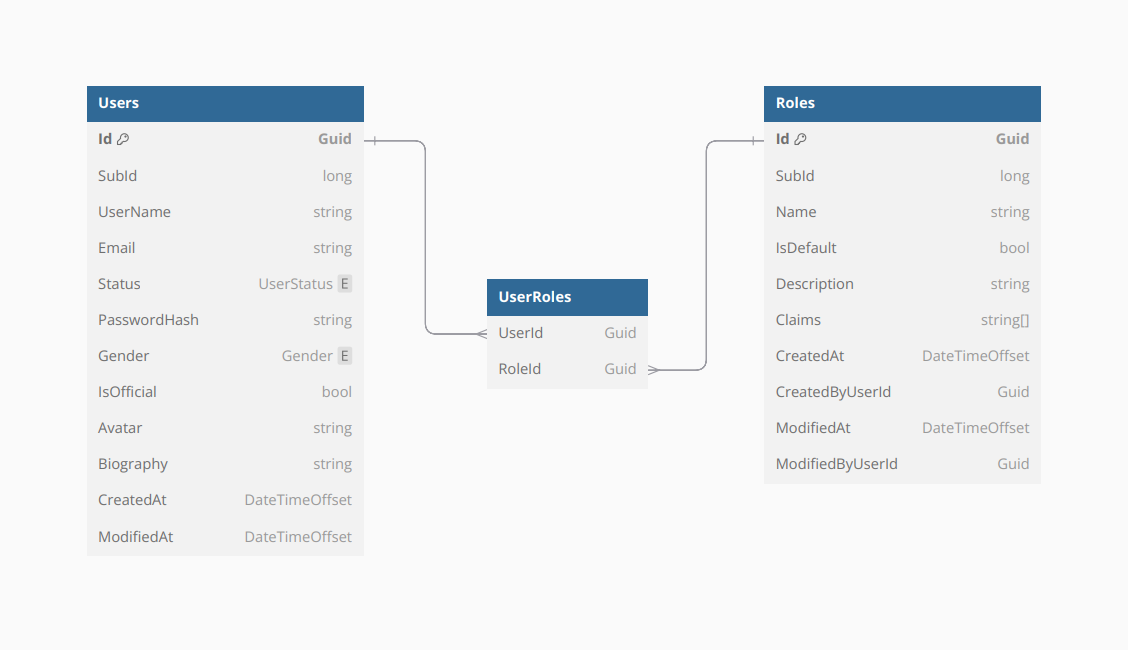
\includegraphics[width=0.85\linewidth]{
            ../figures/service-identity_erd.png
        }
        \caption{Biểu đồ thực thể liên kết Service.Identity}
        \label{fig:service-identity-erd}
    \end{figure}

    \begin{table}[H]
        \begin{tabular}{ |p{3cm}|p{2.5cm}|p{1.6cm}|p{2.2cm}|p{3cm}| }
            \hline
            Tên cột      & Kiểu dữ liệu             & Not Null & Ràng buộc  & Mô tả              \\
            \hline
            Id           & uuid                     & Yes      & Khóa chính & Id người dùng      \\
            \hline
            SubId        & bigint                   & Yes      &            & Sequence           \\
            \hline
            UserName     & text    & Yes      &            & Tên người dùng     \\
            \hline
            Email        & text    & Yes      &            & Địa chỉ Email      \\
            \hline
            Status       & integer                  & Yes      &            & Trạng thái         \\
            \hline
            PasswordHash & text   & Yes      &            & Mật khẩu mã hóa    \\
            \hline
            Gender       & integer                  & Yes      &            & Giới tính          \\
            \hline
            IsOfficial   & boolean                  & Yes      &            & Là chính thức      \\
            \hline
            Avatar       & text   & No       &            & Đường dẫn avatar   \\
            \hline
            Biography    & text   & No       &            & Giới thiệu         \\
            \hline
            CreatedAt    & timestamp & Yes      &            & Thời gian tạo      \\
            \hline
            ModifiedAt   & timestamp & No       &            & Thời gian cập nhật \\
            \hline
        \end{tabular}
        \caption{Mô tả cấu trúc dữ liệu bảng User}
    \end{table}

    \begin{table}[H]
        \begin{tabular}{ |p{3cm}|p{2.5cm}|p{1.6cm}|p{2.2cm}|p{3cm}| }
            \hline
            Tên cột & Kiểu dữ liệu & Not Null & Ràng buộc              & Mô tả         \\
            \hline
            UserId  & uuid         & Yes      & Khóa chính, khóa ngoại & Id người dùng \\
            \hline
            RoleId  & uuid         & Yes      & Khóa chính, khóa ngoại & Id vai trò    \\
            \hline
        \end{tabular}
        \caption{Mô tả cấu trúc dữ liệu bảng UserRole}
    \end{table}

    \begin{table}[H]
        \begin{tabular}{ |p{3cm}|p{2.5cm}|p{1.6cm}|p{2.2cm}|p{3cm}| }
            \hline
            Tên cột      & Kiểu dữ liệu             & Not Null & Ràng buộc  & Mô tả              \\
            \hline
            Id           & uuid                     & Yes      & Khóa chính & Id vai trò         \\
            \hline
            SubId        & bigint                   & Yes      &            & Sequence           \\
            \hline
            Name         & text    & Yes      &            & Tên vai trò        \\
            \hline
            IsDefault    & boolean                  & Yes      &            & Là mặc định        \\
            \hline
            Description  & text   & No       &            & Mô tả              \\
            \hline
            Claims       & text[]                   & Yes      &            & Các quyền          \\
            \hline
            CreatedAt    & timestamp & Yes      &            & Thời gian tạo      \\
            \hline
            CreatedById  & uuid                     & Yes      &            & Id người tạo       \\
            \hline
            ModifiedAt   & timestamp & No       &            & Thời gian cập nhật \\
            \hline
            ModifiedById & uuid                     & No       &            & Id người cập nhật  \\
            \hline
        \end{tabular}
        \caption{Mô tả cấu trúc dữ liệu bảng Role}
    \end{table}

    % 4.2.1
    \subsection{Service Community}
    \begin{figure}[H]
        \centering
        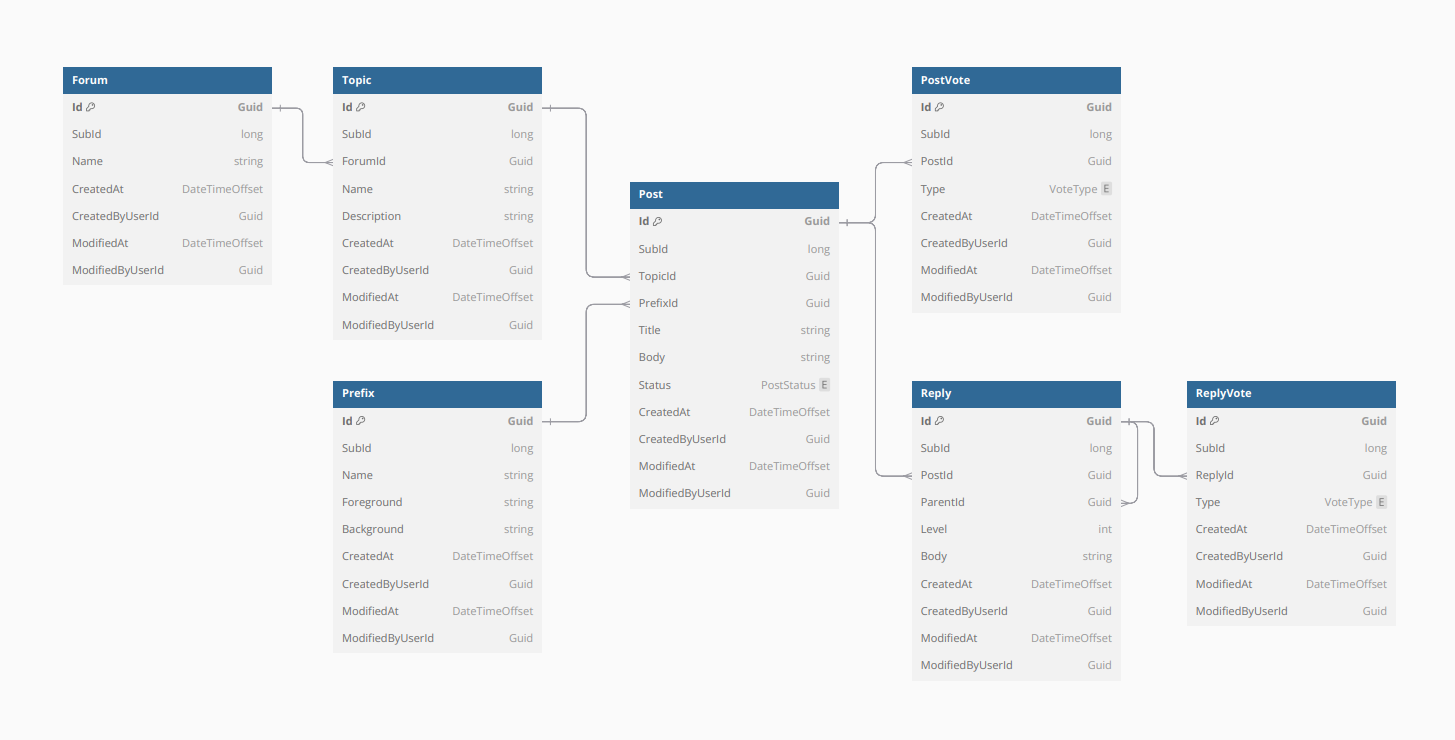
\includegraphics[width=0.85\linewidth]{
            ../figures/service-community_erd.png
        }
        \caption{Biểu đồ thực thể liên kết Service.Community}
        \label{fig:service-community-erd}
    \end{figure}

    \begin{table}[H]
        \begin{tabular}{ |p{3cm}|p{2.5cm}|p{1.6cm}|p{2.2cm}|p{3cm}| }
            \hline
            Tên cột      & Kiểu dữ liệu             & Not Null & Ràng buộc  & Mô tả              \\
            \hline
            Id           & uuid                     & Yes      & Khóa chính & Id diễn đàn        \\
            \hline
            SubId        & bigint                   & Yes      &            & Sequence           \\
            \hline
            Name         & text    & Yes      &            & Tên diễn đàn       \\
            \hline
            CreatedAt    & timestamp & Yes      &            & Thời gian tạo      \\
            \hline
            CreatedById  & uuid                     & Yes      &            & Id người tạo       \\
            \hline
            ModifiedAt   & timestamp & No       &            & Thời gian cập nhật \\
            \hline
            ModifiedById & uuid                     & No       &            & Id người cập nhật  \\
            \hline
        \end{tabular}
        \caption{Mô tả cấu trúc dữ liệu bảng Forum}
    \end{table}

    \begin{table}[H]
        \begin{tabular}{ |p{3cm}|p{2.5cm}|p{1.6cm}|p{2.2cm}|p{3cm}| }
            \hline
            Tên cột      & Kiểu dữ liệu             & Not Null & Ràng buộc  & Mô tả              \\
            \hline
            Id           & uuid                     & Yes      & Khóa chính & Id chủ đề          \\
            \hline
            SubId        & bigint                   & Yes      &            & Sequence           \\
            \hline
            ForumId      & uuid                     & Yes      & Khóa ngoại & Id diễn đàn        \\
            \hline
            Name         & text    & Yes      &            & Tên chủ đề         \\
            \hline
            Description  & text    & No       &            & Mô tả              \\
            \hline
            CreatedAt    & timestamp & Yes      &            & Thời gian tạo      \\
            \hline
            CreatedById  & uuid                     & Yes      &            & Id người tạo       \\
            \hline
            ModifiedAt   & timestamp & No       &            & Thời gian cập nhật \\
            \hline
            ModifiedById & uuid                     & No       &            & Id người cập nhật  \\
            \hline
        \end{tabular}
        \caption{Mô tả cấu trúc dữ liệu bảng Topic}
    \end{table}

    \begin{table}[H]
        \begin{tabular}{ |p{3cm}|p{2.5cm}|p{1.6cm}|p{2.2cm}|p{3cm}| }
            \hline
            Tên cột      & Kiểu dữ liệu             & Not Null & Ràng buộc  & Mô tả              \\
            \hline
            Id           & uuid                     & Yes      & Khóa chính & Id prefix          \\
            \hline
            SubId        & bigint                   & Yes      &            & Sequence           \\
            \hline
            Name         & text    & Yes      &            & Tên prefix         \\
            \hline
            Foreground   & text    & Yes      &            & Màu chữ            \\
            \hline
            Background   & text    & Yes      &            & Màu nền            \\
            \hline
            CreatedAt    & timestamp & Yes      &            & Thời gian tạo      \\
            \hline
            CreatedById  & uuid                     & Yes      &            & Id người tạo       \\
            \hline
            ModifiedAt   & timestamp & No       &            & Thời gian cập nhật \\
            \hline
            ModifiedById & uuid                     & No       &            & Id người cập nhật  \\
            \hline
        \end{tabular}
        \caption{Mô tả cấu trúc dữ liệu bảng Prefix}
    \end{table}

    \begin{table}[H]
        \begin{tabular}{ |p{3cm}|p{2.5cm}|p{1.6cm}|p{2.2cm}|p{3cm}| }
            \hline
            Tên cột      & Kiểu dữ liệu             & Not Null & Ràng buộc  & Mô tả              \\
            \hline
            Id           & uuid                     & Yes      & Khóa chính & Id bài viết        \\
            \hline
            SubId        & bigint                   & Yes      &            & Sequence           \\
            \hline
            TopicId      & uuid                     & Yes      & Khóa ngoại & Id chủ đề          \\
            \hline
            PrefixId     & uuid                     & No       & Khóa ngoại & Id prefix          \\
            \hline
            Title        & text   & Yes      &            & Tiêu đề bài viết   \\
            \hline
            Body         & text                     & Yes      &            & Nội dung bài viết  \\
            \hline
            Status       & int                      & Yes      &            & Trạng thái         \\
            \hline
            CreatedAt    & timestamp & Yes      &            & Thời gian tạo      \\
            \hline
            CreatedById  & uuid                     & Yes      &            & Id người tạo       \\
            \hline
            ModifiedAt   & timestamp & No       &            & Thời gian cập nhật \\
            \hline
            ModifiedById & uuid                     & No       &            & Id người cập nhật  \\
            \hline
        \end{tabular}
        \caption{Mô tả cấu trúc dữ liệu bảng Post}
    \end{table}

    \begin{table}[H]
        \begin{tabular}{ |p{3cm}|p{2.5cm}|p{1.6cm}|p{2.2cm}|p{3cm}| }
            \hline
            Tên cột      & Kiểu dữ liệu             & Not Null & Ràng buộc  & Mô tả              \\
            \hline
            Id           & uuid                     & Yes      & Khóa chính & Id vote bài viết   \\
            \hline
            SubId        & bigint                   & Yes      &            & Sequence           \\
            \hline
            PostId       & uuid                     & Yes      & Khóa ngoại & Id bài viết        \\
            \hline
            Type         & integer                  & Yes      &            & Loại vote          \\
            \hline
            CreatedAt    & timestamp & Yes      &            & Thời gian tạo      \\
            \hline
            CreatedById  & uuid                     & Yes      &            & Id người tạo       \\
            \hline
            ModifiedAt   & timestamp & No       &            & Thời gian cập nhật \\
            \hline
            ModifiedById & uuid                     & No       &            & Id người cập nhật  \\
            \hline
        \end{tabular}
        \caption{Mô tả cấu trúc dữ liệu bảng PostVote}
    \end{table}

    \begin{table}[H]
        \begin{tabular}{ |p{3cm}|p{2.5cm}|p{1.6cm}|p{2.2cm}|p{3cm}| }
            \hline
            Tên cột      & Kiểu dữ liệu             & Not Null & Ràng buộc  & Mô tả              \\
            \hline
            Id           & uuid                     & Yes      & Khóa chính & Id bình luận       \\
            \hline
            SubId        & bigint                   & Yes      &            & Sequence           \\
            \hline
            PostId       & uuid                     & Yes      & Khóa ngoại & Id bài viết        \\
            \hline
            ParentId     & uuid                     & No       & Khóa ngoại & Id bình luận cha   \\
            \hline
            Body         & text                     & Yes      &            & Nội dung bình luận \\
            \hline
            Level        & integer                  & Yes      &            & Cấp độ             \\
            \hline
            CreatedAt    & timestamp & Yes      &            & Thời gian tạo      \\
            \hline
            CreatedById  & uuid                     & Yes      &            & Id người tạo       \\
            \hline
            ModifiedAt   & timestamp & No       &            & Thời gian cập nhật \\
            \hline
            ModifiedById & uuid                     & No       &            & Id người cập nhật  \\
            \hline
        \end{tabular}
        \caption{Mô tả cấu trúc dữ liệu bảng Reply}
    \end{table}

    \begin{table}[H]
        \begin{tabular}{ |p{3cm}|p{2.5cm}|p{1.6cm}|p{2.2cm}|p{3cm}| }
            \hline
            Tên cột      & Kiểu dữ liệu             & Not Null & Ràng buộc  & Mô tả              \\
            \hline
            Id           & uuid                     & Yes      & Khóa chính & Id vote bình luận  \\
            \hline
            SubId        & bigint                   & Yes      &            & Sequence           \\
            \hline
            ReplyId      & uuid                     & Yes      & Khóa ngoại & Id bình luận       \\
            \hline
            Type         & integer                  & Yes      &            & Loại vote          \\
            \hline
            CreatedAt    & timestamp & Yes      &            & Thời gian tạo      \\
            \hline
            CreatedById  & uuid                     & Yes      &            & Id người tạo       \\
            \hline
            ModifiedAt   & timestamp & No       &            & Thời gian cập nhật \\
            \hline
            ModifiedById & uuid                     & No       &            & Id người cập nhật  \\
            \hline
        \end{tabular}
        \caption{Mô tả cấu trúc dữ liệu bảng ReplyVote}
    \end{table}

    % 4.2.1
    \subsection{Service Chat}
    \begin{figure}[H]
        \centering
        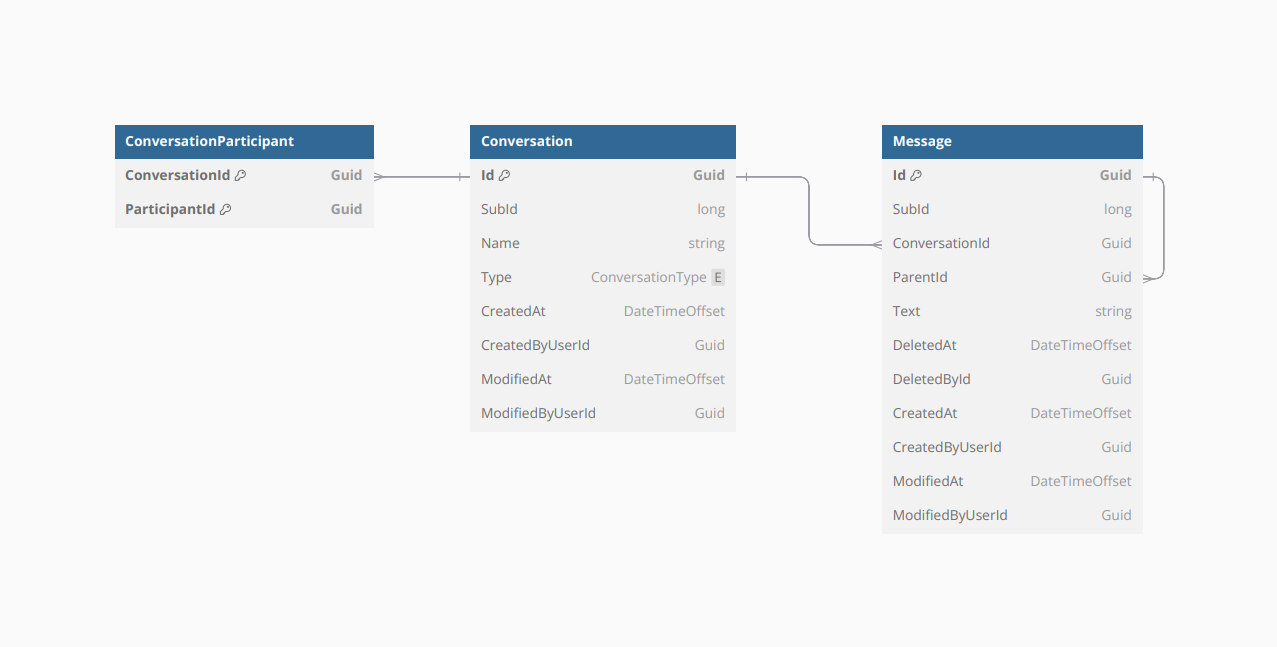
\includegraphics[width=0.85\linewidth]{../figures/service-chat_erd.png}
        \caption{Biểu đồ thực thể liên kết Service.Chat}
        \label{fig:service-chat-erd}
    \end{figure}

    \begin{table}[H]
        \begin{tabular}{ |p{3cm}|p{2.5cm}|p{1.6cm}|p{2.2cm}|p{3cm}| }
            \hline
            Tên cột      & Kiểu dữ liệu             & Not Null & Ràng buộc  & Mô tả              \\
            \hline
            Id           & uuid                     & Yes      & Khóa chính & Id hội thoại       \\
            \hline
            SubId        & bigint                   & Yes      &            & Sequence           \\
            \hline
            Name         & text    & No       &            & Tên hội thoại      \\
            \hline
            Type         & integer                  & Yes      &            & Loại hội thoại     \\
            \hline
            CreatedAt    & timestamp & Yes      &            & Thời gian tạo      \\
            \hline
            CreatedById  & uuid                     & Yes      &            & Id người tạo       \\
            \hline
            ModifiedAt   & timestamp & No       &            & Thời gian cập nhật \\
            \hline
            ModifiedById & uuid                     & No       &            & Id người cập nhật  \\
            \hline
        \end{tabular}
        \caption{Mô tả cấu trúc dữ liệu bảng Conversation}
    \end{table}

    \begin{table}[H]
        \begin{tabular}{ |p{3cm}|p{2.5cm}|p{1.6cm}|p{2.2cm}|p{3cm}| }
            \hline
            Tên cột        & Kiểu dữ liệu             & Not Null & Ràng buộc  & Mô tả              \\
            \hline
            Id             & uuid                     & Yes      & Khóa chính & Id tin nhắn        \\
            \hline
            SubId          & bigint                   & Yes      &            & Sequence           \\
            \hline
            ConversationId & uuid                     & Yes      & Khóa ngoại & Id hội thoại       \\
            \hline
            ParentId       & uuid                     & No       & Khóa ngoại & Id tin nhắn cha    \\
            \hline
            Text           & text   & Yes      &            & Nội dung           \\
            \hline
            CreatedAt      & timestamp & Yes      &            & Thời gian tạo      \\
            \hline
            CreatedById    & uuid                     & Yes      &            & Id người tạo       \\
            \hline
            ModifiedAt     & timestamp & No       &            & Thời gian cập nhật \\
            \hline
            ModifiedById   & uuid                     & No       &            & Id người cập nhật  \\
            \hline
            DeletedAt      & timestamp & No       &            & Thời gian xóa      \\
            \hline
            DeletedById    & uuid                     & No       &            & Id người xóa       \\
            \hline
        \end{tabular}
        \caption{Mô tả cấu trúc dữ liệu bảng Message}
    \end{table}

    \begin{table}[H]
        \begin{tabular}{ |p{3cm}|p{2.5cm}|p{1.6cm}|p{2.2cm}|p{3cm}| }
            \hline
            Tên cột        & Kiểu dữ liệu & Not Null & Ràng buộc  & Mô tả             \\
            \hline
            ConversationId & uuid         & Yes      & Khóa ngoại & Id hội thoại      \\
            \hline
            ParticipantId  & uuid         & Yes      &            & Id người tham gia \\
            \hline
        \end{tabular}
        \caption{Mô tả cấu trúc dữ liệu bảng ConversationParticipant}
    \end{table}

    % 4.2.1
    \subsection{Service Notification}
    \begin{figure}[H]
        \centering
        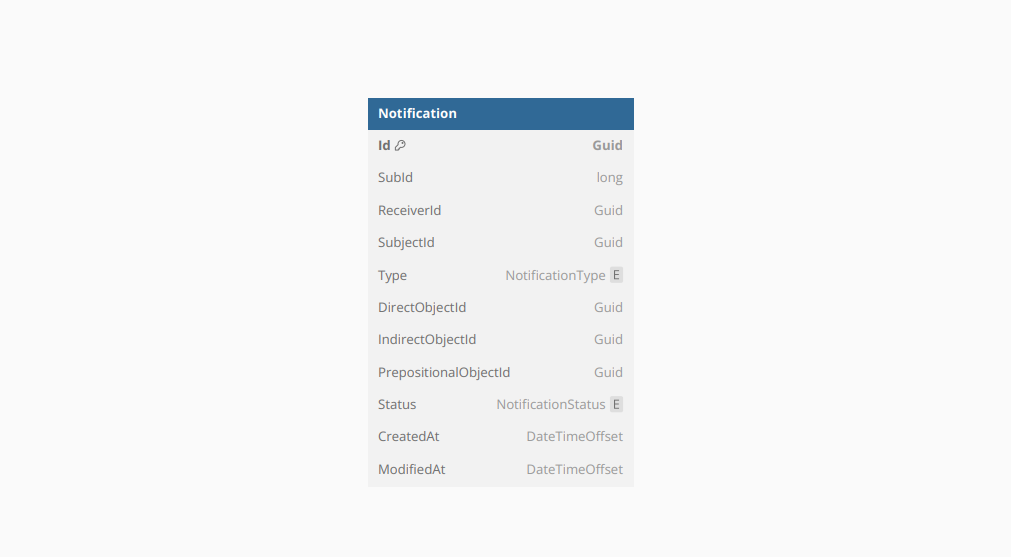
\includegraphics[width=0.85\linewidth]{
            ../figures/service-notification_erd.png
        }
        \caption{Biểu đồ thực thể liên kết Service.Notification}
        \label{fig:service-notification-erd}
    \end{figure}

    \begin{table}[H]
        \begin{tabular}{ |p{4cm}|p{2.5cm}|p{1.6cm}|p{2.2cm}|p{3cm}| }
            \hline
            Tên cột               & Kiểu dữ liệu             & Not Null & Ràng buộc  & Mô tả               \\
            \hline
            Id                    & uuid                     & Yes      & Khóa chính & Id thông báo        \\
            \hline
            SubId                 & bigint                   & Yes      &            & Sequence            \\
            \hline
            ReceiverId            & uuid                     & Yes      &            & Id người nhận       \\
            \hline
            SubjecId              & uuid                     & Yes      &            & Id người tạo        \\
            \hline
            Type                  & integer                  & Yes      &            & Loại thông báo      \\
            \hline
            DirectObjectId        & uuid                     & Yes      &            & Id object trực tiếp \\
            \hline
            IndirectObjectId      & uuid                     & No       &            & Id object gián tiếp \\
            \hline
            PrepositionalObjectId & uuid                     & No       &            & Id object phụ thuộc \\
            \hline
            Status                & integer                  & Yes      &            & Trạng thái          \\
            \hline
            CreatedAt             & timestamp & Yes      &            & Thời gian tạo       \\
            \hline
            ModifiedAt            & timestamp & No       &            & Thời gian cập nhật  \\
            \hline
        \end{tabular}
        \caption{Mô tả cấu trúc dữ liệu bảng Notification}
    \end{table}

    % 4.4
    % \section{Kiểm thử}

    % 4.5
    % \section{Triển khai}
\end{document}